\documentclass[../thesis.tex]{subfiles}
\begin{document}
\chapter{Conclusion}

\label{ch:conclusions}

\section{Applications}

Using the distributedCL class, I have built a few sample applications, that will be described briefly here.

\subsection{Splitting Work} % (fold)
\label{sub:splitting_work}

The first is a simple application to demonstrate the ease in which you can distribute work amongst machines, based in part on the Apple OpenCL Hello World Example \cite{applehelloworld}.

In the program, the GPUs are used to calculate the square of a set of random numbers. The key point is that the buffer is half the size of the data\_barrier, and the work is distributed to two alternative machines, then returned to the source machine. The code required to distribute the work and then gather the data back can be seen in Figure~\ref{fig:split_work}.

\begin{figure}[htbp]
    \centering
    \lstset{language=cpp}
    \begin{lstlisting}
data_barrier<float> barrier = distributedCL.CreateBarrier<float>(DATA_SIZE, DATA_SIZE / 2, context, {0, 1, 2});
...
err = distributedCL.EnqueueWriteBuffer(commands, input, CL_TRUE, 0, DATA_SIZE/2, &barrier, 0, 0, NULL, NULL, NULL, 0, {1});

err = distributedCL.EnqueueWriteBuffer(commands, input, CL_TRUE, 0, DATA_SIZE/2, &barrier, DATA_SIZE/2,  0, NULL, NULL, NULL, 0, {2});
...
data_barrier<float> outputbarrier = distributedCL.CreateBarrier<float>(DATA_SIZE, DATA_SIZE / 2, context, {0, 1, 2});

err = distributedCL.EnqueueReadBuffer(commands, output, CL_TRUE, 0 , DATA_SIZE/2, &outputbarrier, DATA_SIZE/2, 0, NULL, NULL, NULL, 2, {0});
err = distributedCL.EnqueueReadBuffer(commands, output, CL_TRUE, 0 , DATA_SIZE/2, &outputbarrier, 0, 0, NULL, NULL, NULL, 1, {0});
    \end{lstlisting}
    \caption{Splitting Processing}
    \label{fig:split_work}
\end{figure}

In two lines, the data has been split and sent for processing on machine 1 and 2, and in just two more the data has been returned to the main machine.
% subsection splitting_work (end)

\subsection{Non Blocking Enqueue} % (fold)
\label{sub:non_blocking_enqueue}
To demonstrate the ability to generate non blocking command queues with intercommunication, a sample project was built.

The command flow can be seen in Figure~\ref{fig:complex_queue}.

\begin{figure}[htbp]
    \centering
    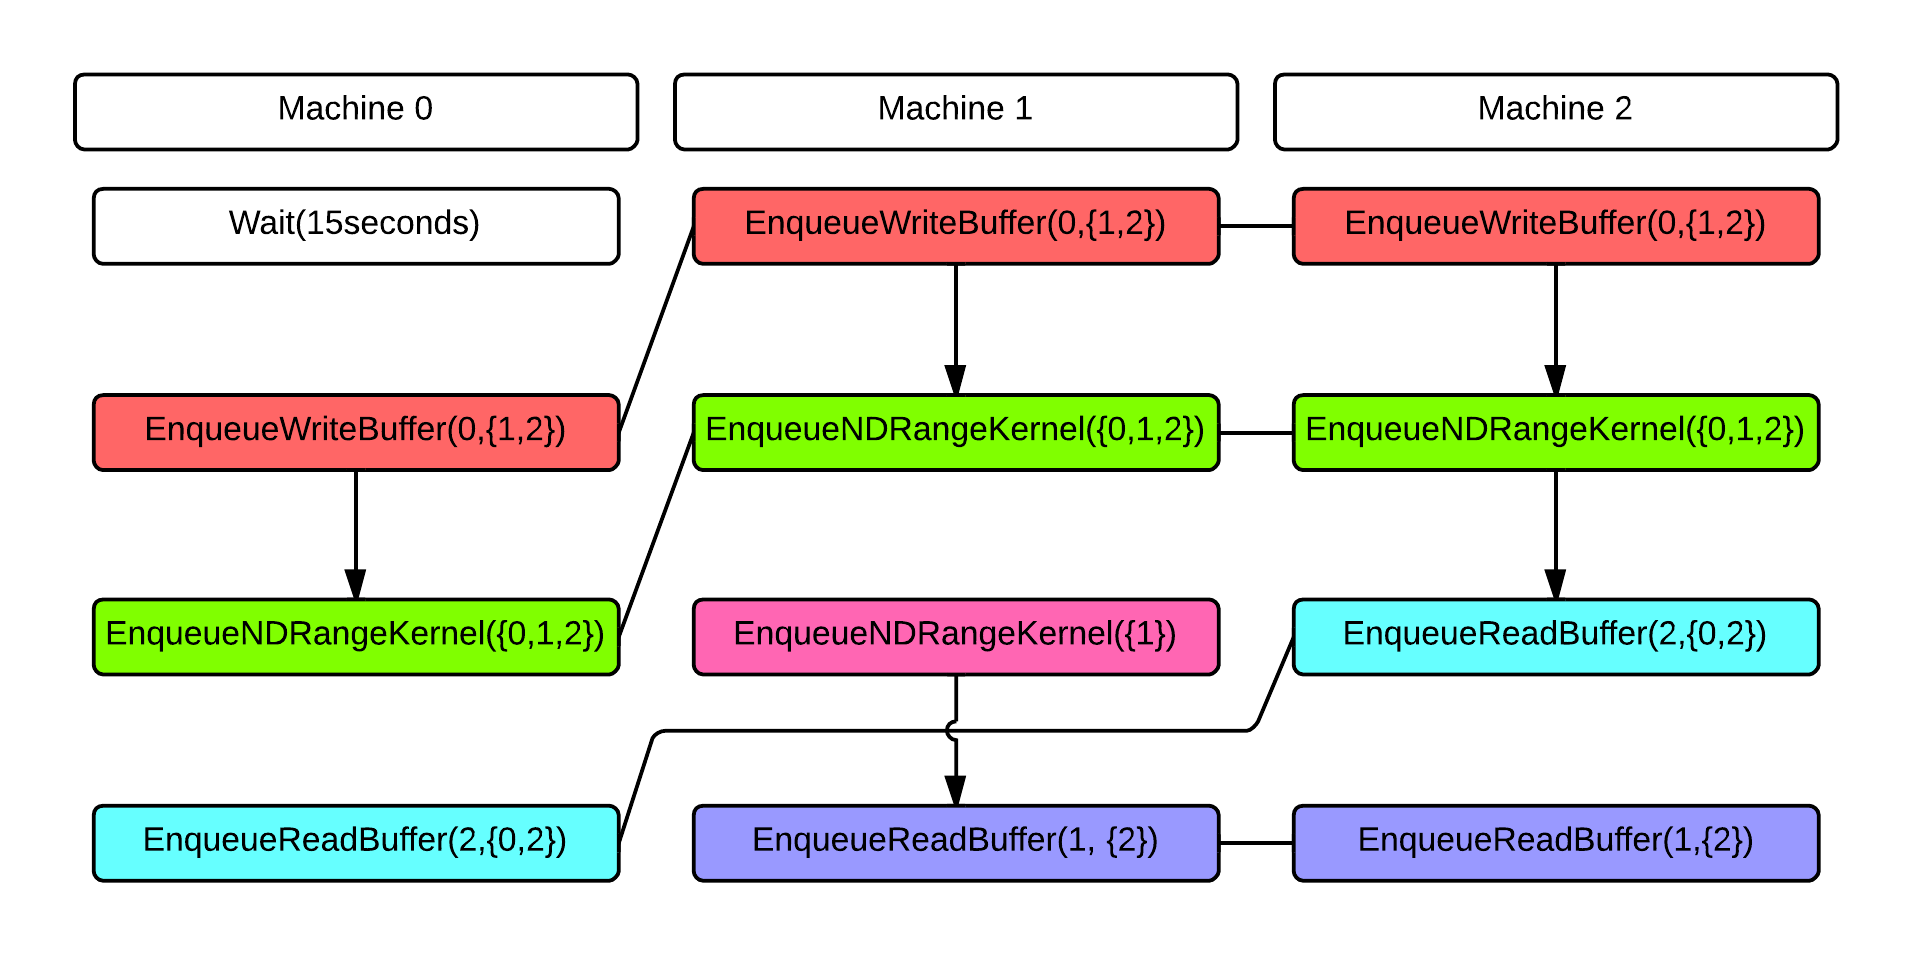
\includegraphics[width=0.95\textwidth]{diagrams/complex_queue.png}
    \caption{Complex Queues}
    \label{fig:complex_queue}
\end{figure}
% subsection non_blocking_enqueue (end)

In the diagram, all of the commands that are the same color represent the same function call. Arrows show that the command is waiting for the previous command to finish, their event was passed as an event wait list. The actual sequence has been truncated, with just a few of the calls shown.

The point of the program is to show that the call of EnqueueWriteBuffer(0,{1,2}) doesn't affect the completion of EnqueueNDRangeKernel{1} and EnqueueReadBuffer(1,{2}). EnqueueReadBuffer will actually finish well ahead of the EnqueueWriteBuffer, because writing will not start until the wait of 15 seconds has been completed. Essentially, it is to show that the queuing commands that involve the transfer of data does not cause blocking, unless you specify it.

\subsection{Heat Transfer} % (fold)
\label{sub:heat_transfer} 

Another example is heat transfer simulations. When running a heat transfer simulation, you may encounter the situation where the simulation size is too large for just a single GPU. In this situation, you partition the data into slices, with an overlap of two rows. Every time you step the simulation, you then exchange the overlapping rows, and step the model. This is demonstrated in Figure~\ref{fig:heat_transfer}.

\begin{figure}[htbp]
    \centering
    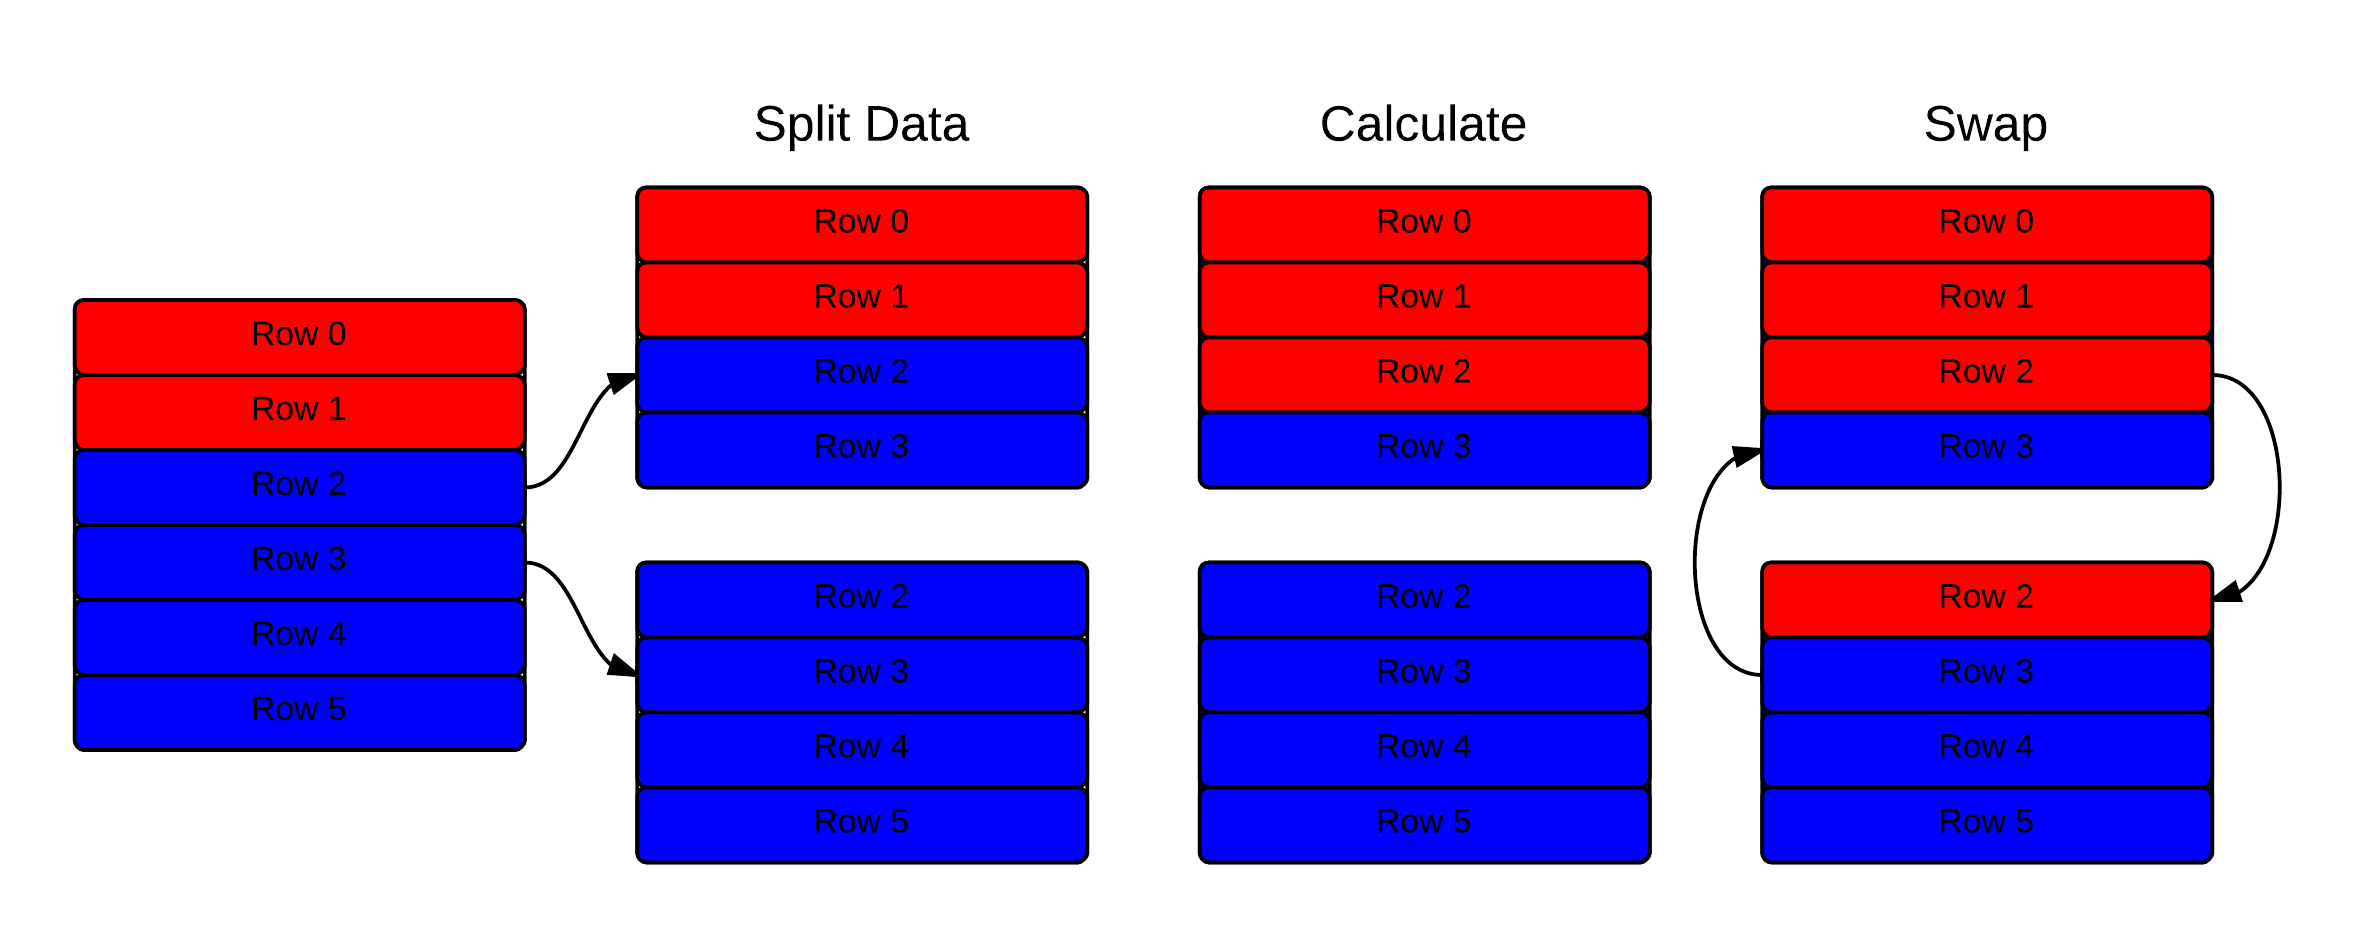
\includegraphics[width=0.95\textwidth]{diagrams/heat_transfer.png}
    \caption{Heat Transfer Example}
    \label{fig:heat_transfer}
\end{figure}

This will be relatively simple once EnqueueCopyBuffer is implemented. Simply step the model, transfer data, step again. Currently, it utilizes a series of separate enqueue reads and enqueue writes.
% subsection heat_transfer (end)

\subsection{Other} % (fold)
\label{sub:other}
    In bioinformatics, there is a large quantity of research dedicated to sequence alignment. Sequence alignment is a method for comparing the similarity of strings, often times representing DNA, RNA, or proteins. One such method for determining sequence alignment is known as the Smith-Waterman algorithm, used for determining optimum local alignment between two compounds. Research has been done into optimizing this algorithm for GPUs, although they are most often CUDA based. Borovska compared the speedup using a variety of methods, and found a significant increase when using GPUs\cite{Borovska:2011:PMS:2023607.2023644}, proving that this algorithm lends itself well to parallel methods.

    Additionally, work has already been undertaken by Yuma Munekawa, Fumihiko Ino, and Kenichi Hagihara to implement the algorithm on a cluster based system, achieving a good speedup \cite{2010}. Already there's been significant speedup, and it would be interesting to see how distributedCL compares to programs designed from the ground up to support this particular algorithm.

    It is important to note, that this program has not been implemented yet, that might alone be a research problem. As such, it can be considered future work. It has been placed under applications as it is not necessary for the development of this project, but an interesting way to see it applied.
% subsection other (end)

\section{Future Work}

There are quite a few ways that the work can be improved in the future. In this section, we will discuss each in turn, reasoning and use.

The first is utilizing MPI\_Comm\_split. Currently, all communication is done over the default communicator, MPI\_COMM\_WORLD. Although it is a negligible worry, there may come a situation where communications clash. By creating a custom communicator for each of the data\_barriers, there can be an assurance that there will be no message clashes during communication. Additionally, this is useful for broadcasting commands; by taking advantage of a custom communicator, commands that send to all machines can be sped up greatly. If there was a data\_barrier shared between 90 machines, the current method would most certainly falter. By using a custom communicator, we could take advantage of MPI's optimizing of broadcast communication.

The next is another MPI based enhancement; make use of MPI derived data types. By utilizing MPI\_Type\_contiguous, we could create a datatype that consists of a single contiguous block, or a chunk. This would be useful solely for simplifying internals, by using these derived datatypes we would reduce the number of parameters we need to keep track of during a send and receive.

Currently some of OpenCL functions do not have distributedCL equivalents; this is because they were added on an as needed basis. In the future, they can be easily added in following the formats provided.

All distributedCL functions currently require a parameter target\_machines, and treat an empty list as all machines. In the future, I'd like to provide an overloaded function without the last parameter that default to all machines.

Another change that would be ideal is thread tracking. As it is, send and receive threads need to either be blocking calls, or have WaitForEvent called for the produced event prior to the call to Finalize. This is because oftentimes MPI\_Finalize will be called by the main thread prior to the send thread finishing the transmission, which leads to errors and poor behavior. By implementing a data member of distributedCL that keeps track of threads, we can became more lax on send and receive completion in functions.

A large change that was not yet implemented is clEnqueueCopyBuffer, and all the changes that implementing it would entail. As far as sending and receiving goes, it stands to reason that the send half would be quite similar to the EnqueueReadBuffer, and the receive half would just be EnqueueWriteBuffer. But it would require quite a few changes to data\_barrier, such as changing it to be a wrapper for a cl\_mem object, (acl\_mem is a handle to a buffer created by clCreateBuffer). In this situation, a data\_barrier would always be passed in place of a buffer object. The only reason it hasn't been implemented is lack of time to overhaul the data\_barrier class and the functions that use it.

In that situation, every buffer object would be associated with an array of a specified data\_type. It would restrict you in the sense that buffers would have to be used for that data type, but it isn't much of a change. Everything would function the same, except the data would always be copied to the array prior to sending.

The biggest change that could possibly happen would be an additional layer of abstraction on top of this. Currently, all data movements must explicitly be thought about by the programmer, it provides a base for building an application that does load balancing for you. The underlying data transfer mechanisms have been defined, but the actual implementation would be very complex.


\section{Summary of Project}
In this project we have designed from a base communication layer an API designed for distributed computing upon networked GPUs. Piece by piece we have abstracted away from the communication layer until we have a product that requires minimal input to target multiple machines. Using threading, a method for non blocking point to point communication has been provided, allowing cross machine enqueueing of commands that require transmission of data, whilst avoiding deadlocks that could be caused by it.

And so we have examined the entirety of distributedCL, an API for distributed computing with OpenCL. Starting from initial considerations of possible approaches for distributed computing, to then actually building it. Covering all the components, from distCL\_event, to data\_barrier, to the actual class distributedCL, all aspects of the design and development have been covered.

The motivations and design of each of these have been described; providing custom events that can be used in the same fashion as cl\_events, a class that manages the exchange of data, and wrapper functions for OpenCL that allow easy targeting of multiple machines.

Thus a base for building complex distributed OpenCL applications has been designed and built, grounds have been laid for future implementations.
\end{document}
